\chapter{外文资料原文}
\label{cha:engorg}

\title{A Survey of Motion Planning and Control Techniques for Self-driving Urban Vehicles}

\textbf{Abstract:} Self-driving vehicles are a maturing technology with the potential to reshape mobility by enhancing the safety, accessibility, efficiency, and convenience of automotive transportation. Safety-critical tasks that must be executed by a self-driving vehicle include planning of motions through a dynamic environment shared with other vehicles and pedestrians, and their robust executions via feedback control. The objective of this paper is to survey the current state of the art on planning and control algorithms with particular regard to the urban setting. A selection of proposed techniques is reviewed along with a discussion of their effectiveness. The surveyed approaches differ in the vehicle mobility model used, in assumptions on the structure of the environment, and in computational requirements. The side-by-side comparison presented in this survey helps to gain insight into the strengths and limitations of the reviewed approaches and assists with system level design choices.

\section{Introduction}
The last three decades have seen steadily increasing research efforts, both in academia and in industry, towards developing driverless vehicle technology. These developments have been fueled by recent advances in sensing and computing technology together with the potential transformative impact on automotive transportation and the perceived societal benefit: In 2014 there were 32,675 traffic related fatalities, 2.3 million injuries, and 6.1 million reported collisions [1]. Of these, an estimated 94\% are attributed to driver error with 31\% involving legally intoxicated drivers, and 10\% from distracted drivers [2]. Autonomous vehicles have the potential to dramatically reduce the contribution of driver error and negligence as the cause of vehicle collisions. They will also provide a means of personal mobility to people who are unable to drive due to physical or visual disability. Finally, for the 86\% of the US work force that commutes by car, on average 25 minutes (one way) each day [3], autonomous vehicles would facilitate more productive use of the transit time, or simply reduce the measurable ill effects of driving stress [4]. Considering the potential impacts of this new technology, it is not surprising that self-driving cars have had a long history. The idea has been around as early as in the 1920s, but it was not until the 1980s that driverless cars seemed like a real possibility. Pioneering work led by Ernst Dickmanns (e.g., [5]) in the 1980s paved the way for the development of autonomous vehicles. At that time a massive research effort, the PROMETHEUS project, was funded to develop an autonomous vehicle. A notable demonstration in 1994 resulting from the work was a 1,600 km drive by the VaMP driverless car, of which 95\% was driven autonomously [6]. At a similar time, the CMU NAVLAB was making advances in the area and in 1995 demonstrated further progress with a 5,000 km drive across the US of which 98\% was driven autonomously [7].

The next major milestone in driverless vehicle technology was the first DARPA Grand Challenge in 2004. The objective was for a driverless car to navigate a 150-mile off-road course as quickly as possible. This was a major challenge in comparison to previous demonstrations in that there was to be no human intervention during the race. Although prior works demonstrated nearly autonomous driving, eliminating human intervention at critical moments proved to be a major challenge. None of the 15 vehicles entered into the event completed the race. In 2005 a similar event was held; this time 5 of 23 teams reached the finish line [8]. Later, in 2007, the DARPA Urban Challenge was held, in which vehicles were required to drive autonomously in a simulated urban setting. Six teams finished the event demonstrating that fully autonomous urban driving is possible [9]. Numerous events and major autonomous vehicle system tests have been carried out since the DARPA challenges. Notable examples include the Intelligent Vehicle Future Challenges from 2009 to 2013 [10], Hyundai Autonomous Challenge in 2010 [11], the VisLab Intercontinental Autonomous Challenge in 2010 [12], the Public Road Urban Driverless- Car Test in 2013 [13], and the autonomous drive of the Bertha-Benz historic route [14]. Simultaneously, research has continued at an accelerated pace in both the academic setting as well as in industry. The Google self-driving car [15] and Tesla’s Autopilot system [16] are two examples of commercial efforts receiving considerable media attention. The extent to which a car is automated can vary from fully human operated to fully autonomous. The SAE J3016 standard [17] introduces a scale from 0 to 5 for grading vehicle automation. In this standard, the level 0 represents a vehicle where all driving tasks are the responsibility of a human driver. Level 1 includes basic driving assistance such as adaptive cruise control, anti-lock braking systems and electronic stability control [18]. Level 2 includes advanced assistance such as hazard-minimizing longitudinal/lateral control [19] or emergency braking [20], [21], often based upon set-based formal control theoretic methods to compute ‘worst-case’ sets of provably collision free (safe) states [22]–[24]. At level 3 the system monitors the environment and can drive with full autonomy under certain conditions, but the human operator is still required to take control if the driving task leaves the autonomous system’s operational envelope. A vehicle with level 4 automation is capable of fully autonomous driving in certain conditions and will safely control the vehicle if the operator fails to take control upon request to intervene. Level 5 systems are fully autonomous in all driving modes. The availability of on-board computation and wireless communication technology allows cars to exchange information with other cars and with the road infrastructure giving rise to a closely related area of research on connected intelligent vehicles [25]. This research aims to improve the safety and performance of road transport through information sharing and coordination between individual vehicles. For instance, connected vehicle technology has a potential to improve throughput at intersections [26] or prevent formation of traffic shock waves [27].

To limit the scope of this survey, we focus on aspects of decision making, motion planning, and control for self-driving cars, in particular, for systems falling into the automation level of 3 and above. For the same reason, the broad field of perception for autonomous driving is omitted and instead the reader is referred to a number of comprehensive surveys and major recent contributions on the subject [28]–[31].

The decision making in contemporary autonomous driving systems is typically hierarchically structured into route planning, behavioral decision making, local motion planning and feedback control. The partitioning of these levels are, however, rather blurred with different variations of this scheme occurring in the literature. This paper provides a survey of proposed methods to address these core problems of autonomous driving. Particular emphasis is placed on methods for local motion planning and control.

The remainder of the paper is structured as follows: In Section II, a high level overview of the hierarchy of decision making processes and some of the methods for their design are presented. Section III reviews models used to approximate the mobility of cars in urban settings for the purposes of motion planning and feedback control. Section IV surveys the rich literature on motion planning and discusses its applicability for self-driving cars. Similarly, Section V discusses the problems of path and trajectory stabilization and specific feedback control methods for driverless cars. Lastly, Section VI concludes with remarks on the state of the art and potential areas for future research.

\section{Overview of the Decision-Makeing Hierarchy Used in Driverless Cars}

In this section we describe the decision making architecture of a typical self-driving car and comment on the responsibilities of each component. Driverless cars are essentially autonomous decision-making systems that process a stream of observations from on-board sensors such as radars, LIDARs, cameras, GPS/INS units, and odometry. These observations, together with prior knowledge about the road network, rules of the road, vehicle dynamics, and sensor models, are used to automatically select values for controlled variables governing the vehicle’s motion. Intelligent vehicle research aims at automating as much of the driving task as possible. The commonly adopted approach to this problem is to partition and organize perception and decision-making tasks into a hierarchical structure. The prior information and collected observation data are used by the perception system to provide an estimate of the state of the vehicle and its surrounding environment; the estimates are then used by the decisionmaking system to control the vehicle so that the driving objectives are accomplished.

The decision making system of a typical self-driving car is hierarchically decomposed into four components (cf. Figure II.1): At the highest level a route is planned through the road network. This is followed by a behavioral layer, which decides on a local driving task that progresses the car towards the destination and abides by rules of the road. A motion planning module then selects a continuous path through the environment to accomplish a local navigational task. A control system then reactively corrects errors in the execution of the planned motion. In the remainder of the section we discuss the responsibilities of each of these components in more detail.

\subsection{Route Planning}
At the highest level, a vehicle’s decision-making system must select a route through the road network from its current position to the requested destination. By representing the road network as a directed graph with edge weights corresponding to the cost of traversing a road segment, such a route can be formulated as the problem of finding a minimum-cost path on a road network graph. The graphs representing road networks can however contain millions of edges making classical shortest path algorithms such as Dijkstra [32] or A* [33] impractical. The problem of efficient route planning in transportation networks has attracted significant interest in the transportation science community leading to the invention of a family of algorithms that after a one-time pre-processing step return an optimal route on a continent-scale network in milliseconds [34], [35]. For a comprehensive survey and comparison of practical algorithms that can be used to efficiently plan routes for both human-driven and self-driving vehicles, see [36].

\subsection{Behavioral Decision Making}
After a route plan has been found, the autonomous vehicle must be able to navigate the selected route and interact with other traffic participants according to driving conventions and rules of the road. Given a sequence of road segments specifying the selected route, the behavioral layer is responsible for selecting an appropriate driving behavior at any point of time based on the perceived behavior of other traffic participants, road conditions, and signals from infrastructure. For example, when the vehicle is reaching the stop line before an intersection, the behavioral layer will command the vehicle to come to a stop, observe the behavior of other vehicles, bikes, and pedestrians at the intersection, and let the vehicle proceed once it is its turn to go. Driving manuals dictate qualitative actions for specific driving contexts. Since both driving contexts and the behaviors available in each context can be modeled as finite sets, a natural approach to automating this decision making is to model each behavior as a state in a finite state machine with transitions governed by the perceived driving context such as relative position with respect to the planned route and nearby vehicles. In fact, finite state machines coupled with different heuristics specific to considered driving scenarios were adopted as a mechanism for behavior control by most teams in the DARPA Urban Challenge [9].

Real-world driving, especially in an urban setting, is however characterized by uncertainty over the intentions of other traffic participants. The problem of intention prediction and estimation of future trajectories of other vehicles, bikes and pedestrians has also been studied. Among the proposed solution techniques are machine learning based techniques, e.g., Gaussian mixture models [37], Gaussian process regression [38], the learning techniques reportedly used in Google’s self-driving system for intention prediction [39], and modelbased approaches for directly estimating intentions from sensor measurements [40], [41].

This uncertainty in the behavior of other traffic participants is commonly considered in the behavioral layer for decision making using probabilistic planning formalisms, such as Markov Decision Processes (MDPs) and their generalizations. For example, [42] formulates the behavioral decision-making problem in the MDP framework. Several works [43]–[46] model unobserved driving scenarios and pedestrian intentions explicitly using a partially-observable Markov decision process (POMDP) framework and propose specific approximate solution strategies.

\subsection{Motion Planning}
When the behavioral layer decides on the driving behavior to be performed in the current context, which could be, e.g., cruise-in-lane, change-lane, or turn-right, the selected behavior has to be translated into a path or trajectory that can be tracked by the low-level feedback controller. The resulting path or trajectory must be dynamically feasible for the vehicle, comfortable for the passenger, and avoid collisions with obstacles detected by the on-board sensors. The task of finding such a path or trajectory is a responsibility of the motion planning system.

The task of motion planning for an autonomous vehicle corresponds to solving the standard motion planning problem as discussed in the robotics literature. Exact solutions to the motion planning problem are in most cases computationally intractable. Thus, numerical approximation methods are typically used in practice. Among the most popular numerical approaches are variational methods that pose the problem as non-linear optimization in a function space, graph-search approaches that construct graphical discretization of the vehicle’s state space and search for a shortest path using graph search methods, and incremental tree-based approaches that incrementally construct a tree of reachable states from the initial state of the vehicle and then select the best branch of such a tree. The motion planning methods relevant for autonomous driving are discussed in greater detail in Section IV.

\subsection{Vehicle Control}
In order to execute the reference path or trajectory from the motion planning system a feedback controller is used to select appropriate actuator inputs to carry out the planned motion and correct tracking errors. The tracking errors generated during the execution of a planned motion are due in part to the inaccuracies of the vehicle model. Thus, a great deal of emphasis is placed on the robustness and stability of the closed loop system.

Many effective feedback controllers have been proposed for executing the reference motions provided by the motion planning system. A survey of related techniques are discussed in detail in Section V.

\section{Modeling For Planning And Control}
In this section we will survey the most commonly used models of mobility of car-like vehicles. Such models are widely used in control and motion planning algorithms to approximate a vehicle’s behavior in response to control actions in relevant operating conditions. A high-fidelity model may accurately reflect the response of the vehicle, but the added detail may complicate the planning and control problems. This presents a trade-off between the accuracy of the selected model and the difficulty of the decision problems. This section provides an overview of general modeling concepts and a survey of models used for motion planning and control.

Modeling begins with the notion of the vehicle configuration, representing its pose or position in the world. For example, configuration can be expressed as the planar coordinate of a point on the car together with the car’s heading. This is a coordinate system for the configuration space of the car. This coordinate system describes planar rigid-body motions (represented by the Special Euclidean group in two dimensions, SE(2)) and is a commonly used configuration space [47]–[49]. Vehicle motion must then be planned and regulated to accomplish driving tasks and while respecting the constraints introduced by the selected model.

\subsection{The Kinematic Single-Track Model}
In the most basic model of practical use, the car consists of two wheels connected by a rigid link and is restricted to move in a plane [48]–[52]. It is assumed that the wheels do not slip at their contact point with the ground, but can rotate freely about their axes of rotation. The front wheel has an added degree of freedom where it is allowed to rotate about an axis normal to the plane of motion. This is to model steering. These two modeling features reflect the experience most passengers have where the car is unable to make lateral displacement without simultaneously moving forward. More formally, the limitation on maneuverability is referred to as a nonholonomic constraint [47], [53]. The nonholonomic constraint is expressed as a differential constraint on the motion of the car. This expression varies depending on the choice of coordinate system. Variations of this model have been referred to as the car-like robot, bicycle model, kinematic model, or single track model.

The following is a derivation of the differential constraint in several popular coordinate systems for the configuration. In reference to Figure \ref{fig:kinematics}, the vectors $p_r$ and $p_f$ denote the location of the rear and front wheels in a stationary or inertial coordinate system with basis vectors $(\hat{e}_x, \hat{e}_y, \hat{e}_z)$. The heading $\theta$ is an angle describing the direction that the vehicle is facing. This is defined as the angle between vectors $\hat{e}_x$ and $p_f-p_r$.

The motion of the points $p_r$ and $p_f$ must be collinear with the wheel orientation to satisfy the no-slip assumption. Expressed as an equation, this constraint on the rear wheel is
\begin{equation}
(\dot{p}_r\cdot \hat{e}_y)\cos(\theta)-(\dot{p}_r\cdot \hat{e}_x)\sin(\theta)=0,
\end{equation}
and for the front wheel:
\begin{equation}
(\dot{p}_f\cdot \hat{e}_y)\cos(\theta+\delta)-(\dot{p}_f\cdot \hat{e}_x)\sin(\theta+\delta)=0.
\end{equation}

This expression is usually rewritten in terms of the componentwise motion of each point along the basis vectors. The motion of the rear wheel along the $\hat{e}_x$-direction is $x_r := p_r\cdot\hat{e}_x$. Similarly, for $\hat{e}_y$-direction, $y_r:=p_r\cdot \hat{e}_y$. The forward speed is $v_r:=\dot{p}_r\cdot(p_f-p_r)/\|(p_f-p_r)\|$, which is the magnitude of $\dot{p}_r$ with the correct sign to indicate forward or reverse driving. In terms of the scalar quantities $x_r$, $y_r$, and $\theta$, the differential constraint is
\begin{align}
\begin{split}
\dot{x}_r&= v_r\cos(\theta),\\
\dot{y}_r&= v_r\sin(\theta),\\
\dot{\theta}&=\frac{v_r}{l}\tan(\delta).
\end{split}
\end{align}
Alternatively, the differential constraint can be written in terms the motion of $p_f$,
\begin{align}
\begin{split}
\dot{x}_f&= v_f\cos(\theta),\\
\dot{y}_f&= v_f\sin(\theta),\\
\dot{\theta}&=\frac{v_f}{l}\tan(\delta).
\end{split}
\label{eq:vf}
\end{align}
where the front wheel forward speed $v_f$ is now used. The front wheel speed, $v_f$ , is related to the rear wheel speed by
\begin{equation}
\frac{v_r}{v_f}=\cos(\delta).
\end{equation}

The planning and control problems for this model involve selecting the steering angle $\delta$ within the mechanical limits of the vehicle $\delta\in [\delta_{\min}, \delta_{\max}]$, and forward speed $v_r$ within an acceptable range, $v_r\in [v_{\min}, v_{\max}]$.

A simplification that is sometimes utilized, e.g. [56], is to select the heading rate $\omega$ instead of steering angle $\delta$. These quantities are related by
\begin{equation}
\delta=\arctan(\frac{l\omega}{v_r})
\end{equation}
simplifying the heading dynamics to
\begin{equation}
\dot{\theta}=\omega, \quad \omega\in [\frac{v_r}{l}\tan(\delta_{\min}, \frac{v_r}{l}\tan(\delta_{\max})]
\end{equation}
In this situation, the model is sometimes referred to as the unicycle model since it can be derived by considering the motion of a single wheel. An important variation of this model is the case when $v_r$ is fixed. This is sometimes referred to as the Dubins car, after Lester Dubins who derived the minimum time motion between to points with prescribed tangents [57].Another notable variation is the Reeds-Shepp car for which minimum length paths are known when $v_r$ takes a single forward and reverse speed [58]. These two models have proven to be of some importance to motion planning and will be discussed further in Section IV.

The kinematic models are suitable for planning paths at low speeds (e.g. parking maneuvers and urban driving) where inertial effects are small in comparison to the limitations on mobility imposed by the no-slip assumption. A major drawback of this model is that it permits instantaneous steering angle changes which can be problematic if the motion planning module generates solutions with such instantaneous changes. Continuity of the steering angle can be imposed by augmenting (\ref{eq:vf}), where the steering angle integrates a commanded rate as in [49]. Equation (\ref{eq:vf}) becomes
\begin{align}
\begin{split}
\dot{x}_f&= v_f\cos(\theta),\\
\dot{y}_f&= v_f\sin(\theta),\\
\dot{\theta}&=\frac{v_f}{l}\tan(\delta),\\
\dot{\delta}&=v_{\delta}.
\end{split}
\end{align}

In addition to the limit on the steering angle, the steering rate can now be limited: $v_{\delta}\in [\dot{\delta}_{\min},\dot{\delta}_{\max}]$. The same problem can arise with the car’s speed vr and can be resolved in the same way. The drawback to this technique is the increased dimension of the model which can complicate motion planning and control problems. The choice of coordinate system is not limited to using one of the wheel locations as a position coordinate. For models derived using principles from classical mechanics it can be convenient to use the center of mass as the position coordinate as in [59], [60], or the center of oscillation as in [61], [62].

\chapter{外文资料的调研阅读报告或书面翻译}

\title{城市道路自动驾驶车辆运动计划和控制研究综述}

{\heiti 摘要:} 自动驾驶车是一种成熟的技术,通过提高汽车运输的安全性,可及性,效率和便利性,有可能重塑人们的出行方式。 自驾车必须在确保安全的前提下执行任务,包括通过与其他车辆和行人共享的动态环境进行动作规划,以及通过反馈控制可靠地执行动作。 本文的目的是调查目前的规划和控制算法的现状,特别是在城市环境中。本文对部分所提出的技术进行了综述,并讨论了其有效性。 所调查的方法在所使用的车辆移动性模型,环境结构假设和计算要求方面不同。 本次调查中的并列比较有助于深入了解经过调查的方法的优势和局限性,并辅助系统级设计选择。

\section{介绍}

过去三十年来,学术界和工业界都在不断开展无人驾驶技术的研究工作。传感和计算技术的最新进展,无人驾驶技术对汽车运输的潜在转变及其社会效益,推动了这项技术的发展:2014年有交通相关死亡人员32,675人,其中230万人受伤,610万起交通事故被报道[1]。其中,估计有94\%的事故是由驾驶员操作失误造成,31\%涉及饮酒的驾驶员,10\%涉及分心的驾驶员[2]。自动驾驶车有可能大大减少因驾驶员犯错和疏忽而造成的事故。它们还将为由于身体或视觉残疾而无法驾驶的人提供私人交通工具。最后,全美工作人口86\%的人每天平均花25分钟(单程)的时间乘汽车上下班,自动驾驶车将有助于更有效地利用通勤时间,或简单地减少驾驶压力带来的不良影响[4]。

考虑到这种新技术的潜在影响,自驾车已经有悠久的历史。这个想法早在20世纪20年代就已经存在,但直到20世纪80年代,无人驾驶的汽车才真正成为可能。 20世纪80年代由恩斯特·迪克曼(Ernst Dickmanns)(例如[5])领导的开创性工作为无人车的开发铺平了道路。那时候,PROMETHEUS项目的大量研究力量投入了无人车的研发。 1994年,由VaMP开发的无人驾驶汽车驾驶1600公里,其中95\%是自主驾驶[6]。在同一时期,CMU NAVLAB正在该领域取得进展,并在1995年展示了进一步的进展,在5000公里穿越美国的车程中,98\%是自主驾驶[7]。

无人驾驶汽车技术的下一个重大里程碑是2004年第一次DARPA大挑战赛。比赛目标是让无人驾驶汽车尽快通过150英里的越野赛道。与以前的展示相比,这是一个重大的挑战,因为在比赛中不会有人为的干预。虽然以前的工作能实现几乎自主的驾驶,但在关键时刻消除人为干预被证明是一个重大的挑战。15辆车中没有一辆完成比赛。 2005年举办了类似的活动;这一次,23支队伍中有5个到达了终点线[8]。后来,2007年,DARPA城市挑战赛举行,车辆被要求在模拟城市环境中自主驾驶。六个小组完成了这一比赛,表明完全自主的城市驾驶是可能的[9]。

自从DARPA挑战以来,全世界已经进行了许多比赛和较大的无人车系统测试。值得注意的例子包括2009年至2013年的智能车辆未来挑战赛[10],2010年的现代汽车无人车挑战赛[11],2010年的VisLab洲际无人车挑战赛[12],2013年的城市无人驾驶汽车公路测试[13],以及Bertha-Benz路线的自主驾驶测试[14]。同时,在学术环境的改善和行业发展的驱动下,无人车研究工作进展顺利。 Google自驾车[15]和特斯拉的自动驾驶仪系统[16]是获得广泛关注的商业活动的两个例子。

汽车自动化的程度可以从完全由人操作到完全自主操作。 SAE J3016标准[17]引入了从0到5的等级分级车辆自动化程度。在这个标准中,0级代表车辆所有驾驶任务都是人类驾驶员完成。1级包括基本驾驶辅助,如自适应巡航控制,防抱死制动系统和电子稳定控制[18]。2级包括高级辅助系统,如危害最小化纵向/横向控制[19]和紧急制动[20],[21],这些系统通常基于预先设定形式的控制理论来计算“最坏情况” (安全)状态[22] - [24],确保车辆无碰撞。在3级系统中,系统对行车环境进行监控,并且可以在某些条件下完全自主地运行,但如果驾驶任务离开自主系统的操作范围,则仍然需要操作人员进行控制。具有4级自动化的车辆能够在某些条件下完全自主驾驶,并且如果操作者没有根据要求进行干预,仍可以安全地控制车辆。 5级系统在所有驾驶模式下都是完全自主的。

车载计算和无线通信技术的可用性允许汽车与其他车辆和道路基础设施交换信息,引发了与之密切相关的智能网联车技术的研究[25]。这方面研究旨在通过个别车辆之间的信息共享和协调来提高道路运输的安全性和性能。例如,网联车技术有可能改善交叉点处的吞吐量[26]或阻止交通冲击波的形成[27]。

为了限制本次调查的范围,我们专注于自主驾驶汽车的决策,运动规划和控制方面,特别是对于3级及以上的自动化系统。出于同样的原因,自动驾驶车的感知技术被忽略,读者可以参考关于这一主题的一些综述和近期的重要进展[28] - [31]。

当代自主驾驶系统的决策通常分层次地组织成路线规划,行为决策,局部运动规划和反馈控制。然而,文献中有许多不同的划分,因此对决策级别的划分相当模糊。本文对于解决这些自主驾驶核心问题所提出的方法展开了调查,特别强调局部运动规划和控制的方法。

本文的其余部分结构如下:第二部分对决策过程层次进行了概述,展示了部分设计方法。第三节回顾了用于在城市环境中估计汽车的移动性的模型,以便进行运动规划和反馈控制的研究。第四节调查有关运动规划的丰富文献,并讨论其对自驾车的适用性。同样,第五节讨论了无人驾驶汽车的路径和轨迹稳定问题以及具体的反馈控制方法。最后,第六部分总结了并评述了研究现状和未来研究方向。


\section{无人车决策层次概述}

在本节中,我们将描述典型自驾车的决策层次,并对每个部分的功能进行描述。无人驾驶汽车本质上是自动决策系统,可处理来自车载传感器(如雷达,LIDAR,摄像机,GPS / INS单元和测距仪)的观测数据流。这些观察结果以及关于道路网络的现有知识,道路规则,车辆动力学和传感器模型被用于自动选择控制车辆运动的控制变量的值。智能车辆研究旨在尽可能多地自动化驾驶任务。该问题通常采用的方法是将感知和决策任务分解和组织成一个层次结构。感知系统使用先前的信息和收集的观测数据来提供车辆状态及对周围环境的估计,然后由决策系统使用估计来控制车辆,从而完成驾驶目标。

典型自驾车的决策系统被分层分解为四个组成部分(参见图\ref{fig:decision}):在最高层,路线是通过道路网计划的。这之后是一个行为层,决定了一个局部的驾驶任务,逐渐将汽车导向目的地,并兼顾交通规则。运动规划模块然后在通行环境中规划一条连续路径以完成局部导航任务。最后由控制系统在运动的执行中反馈性地纠正错误。在本节的其余部分,我们将更详细地讨论每个部分的功能。

\begin{figure}
\centering
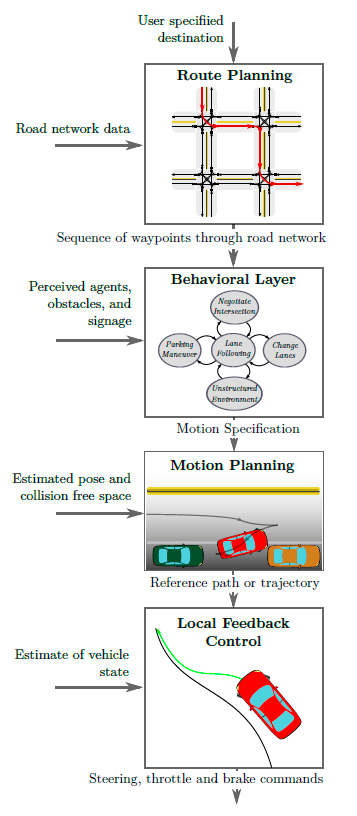
\includegraphics[width=8cm]{decision.png}
\caption{无人车决策层级图}
\caption*{目的地作为路径规划层的输入,生成路网上的路径。行为决策层根据该路径和周围环境,生成一列指向目的地的具体行动。运动规划层进而规划出完成该行动的可行路径。反馈控制调整执行变量以纠正执行参考路径中的错误。}
\label{fig:decision}
\end{figure}

\subsection{路径规划}
在最高级别,车辆的决策系统必须选择通过道路网从当前位置到所要求的目的地的路线。通过将道路网络表示为具有与穿越该路段的成本相对应的赋权有向图,可以将路径规划问题转化为在道路网络图上找到最小成本路径的问题。然而,代表道路网络的图形可以包含数百万条边,使得经典的最短路径算法(如Dijkstra [32]或A * [33])不切实际。运输网络中高效路线规划的问题引起了运输科学界的极大兴趣,研究者发明了一系列算法,经过一次性预处理步骤,可以在几毫秒内在大陆规模的网络上返回最佳路径[34],[35]。对于可用于有效规划驾驶员驾驶和自动驾驶车路线的实际算法的综合调查和比较,参见[36]。

\subsection{行为决策}
在找到路线之后,无人车必须能够根据交通规则,导航所选择的路线,并与其他交通参与者进行交互。给定指示所选路线的路段的序列,行为决策层负责根据其他交通参与者的感知行为,路况和基础设施的信号在任意时间点选择合适的驾驶行为。例如,当车辆在交叉口前到达停车线时,行为层将命令车辆停下来,观察交叉路口处的其他车辆,自行车和行人的行为,并当轮到本车运行时发出运行指令。驾驶手册规定了具体驾驶环境的定性动作。由于驾驶环境和每个环境中可用的行为都可以被建模为有限集,自动化这种决策的自然方法是将每个行为建模成有限状态机中的状态,其中转移由感知到的驾驶环境控制,如本车相对于计划路线和附近车辆的位置。事实上,DARPA城市挑战中大多数团队都采用了有限状态机与特定于驾驶场景的不同启发式搜索[9]作为行为控制机制。

然而,现实世界的驾驶,特别是在城市中,其他交通参与者的意图不确定。研究者们还研究了其他车辆,自行车和行人未来轨迹的意图预测和估计问题。所提出的解决方案是基于机器学习的技术,例如高斯混合模型[37],高斯过程回归[38](这种方法被用于Google自主驾驶系统中意图预测的学习[39]),以及基于模型的直接从传感器测量数据估计意图的方法[40],[41]。

其他交通参与者的行为中的这种不确定性在行为决策层中通常建模为概率模型(例如马尔可夫决策过程(MDP))。例如,[42]在MDP框架中制定行为决策。一些工作[43] - [46]将未观察到的驾驶场景和行人意图显式建模为部分可观察的马尔可夫决策过程(POMDP),并提出具体的求近似解的策略。

\subsection{运动规划}
当行为层决定在当前环境中执行的驾驶行为,例如跟驰,换道或右转时,所选择的行为必须被转换为路径或轨迹,才可以由低级反馈控制器跟踪。所得到的路径或轨迹必须对于车辆而言是动态可行的,对于乘客来说舒适,并且避免与车载传感器检测到的障碍物的碰撞。找到这样的路径或轨迹是运动规划系统的任务。

无人车的运动规划任务与机器人控制相关文献中讨论的求解标准运动规划的问题密切相关。在大多数情况下,运动规划问题的精确解决方案在计算上是不可行的。因此,在实践中通常使用数值近似方法。最常用的数值方法有变分法、图搜索发和增量树法等。其中变分法将轨迹求解问题转化为函数空间中的非线性优化问题;图搜索方法将构成车辆状态空间的道路拓扑图离散化并搜索最短路径;增量树法从车辆的初始状态逐渐构建可达状态树,然后选择这样一棵树的最佳分支。自动驾驶相关的运动规划方法在第四节中有更详细的讨论。

\subsection{车辆控制}
为了执行运动规划系统确定的参考路径或轨迹,无人车使用反馈控制器来选择适当的执行器输入以执行计划的运动和纠正跟踪误差。 执行计划运动期间产生的跟踪误差部分原因在于车辆模型的不准确。 因此,闭环系统的鲁棒性和稳定性非常重要。

研究者们已经设计了许多有效的反馈控制器,来执行由运动规划系统提供的参考路径或轨迹。 相关技术在第五节中有详细的讨论。

\section{无人车运动模型}
在本节中,我们将调查最常用的车辆运动模型。这些模型被广泛用于控制和运动规划算法中,来近似车辆的行为,响应相关操作条件下的控制动作。高保真模型可以准确反映车辆对控制量输入的响应,但是附加的细节可能使计划和控制问题复杂化。这提供了所选模型的准确性与决策问题的难度之间的权衡。本节概述了一般建模概念和运动规划和控制模型。

建模从车辆配置的概念开始,代表其在世界上的姿势或位置。例如,配置可以表示为汽车上的点与汽车的航向的平面坐标。这是汽车配置空间的坐标系。该坐标系描述平面刚体运动(由特殊欧几里德组在两维中表示,SE(2)),并且是常用的配置空间[47] - [49]。车辆运动的规划和调整必须在遵循所选模型引入的限制的前提下,完成驾驶任务。

\subsection{单轨道运动学模型}
在实际使用的最基本模型中,汽车由两个通过刚性连杆连接的轮子组成,并被限制在一个平面上移动[48] - [52]。 假设车轮在与地面的接触点处不会滑动,而可以绕其旋转轴线自由旋转。 前轮具有附加的自由度,允许其绕垂直于运动平面的轴线旋转,以对转向进行建模。 该模型的这两个特征反映了大多数乘客在不同时前进的情况下不能进行横向位移的经验。 更正式地说,这种机动性的限制被称为非完整约束[47],[53]。 非完整约束被表示为对汽车运动的差分约束。 该表达式取决于坐标系的选择。 该模型的各种变种通常被称为类车机器人,自行车模型,运动模型或单轨道模型。

以下是用于配置的几个常用坐标系中差分约束的推导。 参考图\ref{fig:kinematics},矢量$p_r$和$p_f$表示后轮和前轮在具有基矢量$(\hat{e}_x, \hat{e}_y, \hat{e}_z)$的静止或惯性坐标系中的位置。朝向角$\theta$是描述车辆所面向的方向的角度,定义为向量$\hat{e}_x$和$p_f-p_r$之间的角度。
\begin{figure}
\centering
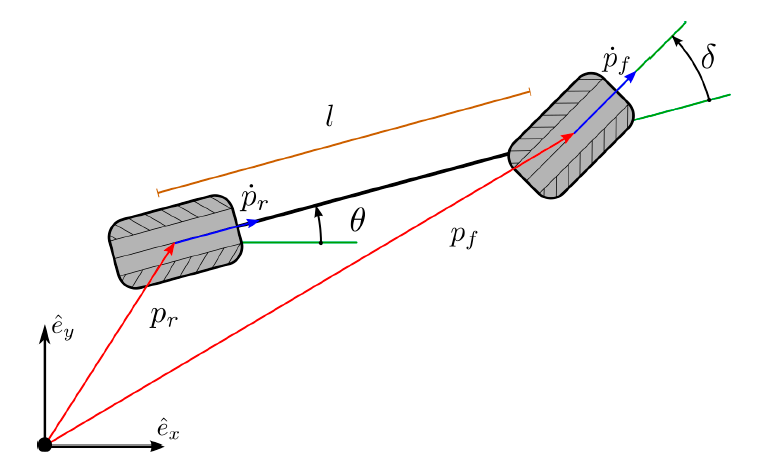
\includegraphics[width=13cm]{kinematics.png}
\caption{单轨道运动学模型图}
\caption*{$p_r$与$p_f$分别为后轮、前轮与地面的触点,$\theta$是车辆朝向角。$p_r$与$p_f$对时间的导数的方向受到非完整性约束的限制,如图中蓝色箭头所示。$\delta$是前轮导向角。}
\label{fig:kinematics}
\end{figure}

下面将对于包含朝向角$\theta$,点$p_r$的运动,点$p_f$的运动的坐标系导出差分约束。

为了满足接触点不滑动的约束,点$p_r$,$p_f$的运动必须与轮子的朝向共线,对后轮,该约束表示为
\begin{equation}
(\dot{p}_r\cdot \hat{e}_y)\cos(\theta)-(\dot{p}_r\cdot \hat{e}_x)\sin(\theta)=0,
\end{equation}
对前轮,有
\begin{equation}
(\dot{p}_f\cdot \hat{e}_y)\cos(\theta+\delta)-(\dot{p}_f\cdot \hat{e}_x)\sin(\theta+\delta)=0.
\end{equation}
该表达式通常被重写为关于基向量的分量形式。后轮运动在$\hat{e}_x$方向的分量为$x_r := p_r\cdot\hat{e}_x$,在$\hat{e}_y$方向为$y_r:=p_r\cdot \hat{e}_y$。前进速度为$v_r:=\dot{p}_r\cdot(p_f-p_r)/\|(p_f-p_r)\|$,即$\dot{p}_r$的模长乘上表示方向的符号。关于标量$x_r$,$y_r$和$\theta$,差分约束表示为
\begin{align}
\begin{split}
\dot{x}_r&= v_r\cos(\theta),\\
\dot{y}_r&= v_r\sin(\theta),\\
\dot{\theta}&=\frac{v_r}{l}\tan(\delta).
\end{split}
\end{align}
同样,对于点$p_f$的运动也具有差分约束
\begin{align}
\begin{split}
\dot{x}_f&= v_f\cos(\theta),\\
\dot{y}_f&= v_f\sin(\theta),\\
\dot{\theta}&=\frac{v_f}{l}\tan(\delta).
\end{split}
\label{eq:vf}
\end{align}
其中,前轮速度$v_f$与后轮速度有关系
\begin{equation}
\frac{v_r}{v_f}=\cos(\delta).
\end{equation}

对该车辆模型的规划和控制需要决定前轮导向角$\delta\in [\delta_{\min}, \delta_{\max}]$和前进速度$v_r\in [v_{\min}, v_{\max}]$。

一个常用的简化,如在[56]中用到的,是选择航向率$\omega$,而不是导向角$\delta$。二者存在关系
\begin{equation}
\delta=\arctan(\frac{l\omega}{v_r})
\end{equation}
这将朝向的运动简化为
\begin{equation}
\dot{\theta}=\omega, \quad \omega\in [\frac{v_r}{l}\tan(\delta_{\min}, \frac{v_r}{l}\tan(\delta_{\max})]
\end{equation}
这种模型有时被称为单轮车模型,因为它可以通过考虑单个车轮的运动而得出。

单轨道运动模型的一个重要变种是固定$v_r$的情况。 这有时被称为杜宾斯车,以莱斯特·杜宾斯(Lester Dubins)命名,他在规定切线的情形下得出了两点之间的最短时间运动[57]。另一个重要变种是Reed-Shepp车,当$v_r$取单值的正向和反向速度时,可以求出最小长度的路径[58]。 这两个模型已被证明对运动规划具有重要意义,并将在第四节进一步讨论。

运动学模型适用于低速情形,例如停车机动和城市驾驶。在该情形下车的惯性较小,不足以打破车轮不打滑的假设。该模型的主要缺点是它允许转向角度瞬间变化。如果运动计划模块要求产生这种瞬时变化,这将是有问题的。

转向角的连续性可以通过改进(\ref{eq:vf})来实现,其中转向角是转角速率的积分,如[49]所示。 方程式(\ref{eq:vf})变为
\begin{align}
\begin{split}
\dot{x}_f&= v_f\cos(\theta),\\
\dot{y}_f&= v_f\sin(\theta),\\
\dot{\theta}&=\frac{v_f}{l}\tan(\delta),\\
\dot{\delta}&=v_{\delta}.
\end{split}
\end{align}
除了对导向角的连续性限制,转角变化率也可以引入约束$v_{\delta}\in [\dot{\delta}_{\min},\dot{\delta}_{\max}]$。同样的问题也会出现在速度控制上。可以通过引入加速度保证速度控制的连续性。这种方法的缺点在于增加了模型的维数,将运动计划与控制问题变得更为复杂。

坐标系的选择不限于使用一个车轮位置作为位置坐标。 对于使用经典力学原理得出的模型,可以使用质心作为位置坐标,如[59],[60]或使用振荡中心,如[61],[62]。